\chapter{
ماشین لباسشویی
}
\section{
طراحی کلی
}
این مدار کنترل کننده یک مدار ترتیبی ساده است که در شکل زیر حالت‌های آن آمده است. 

\begin{figure}[h!]
    \centering
    

\tikzset{every picture/.style={line width=0.75pt}} %set default line width to 0.75pt        

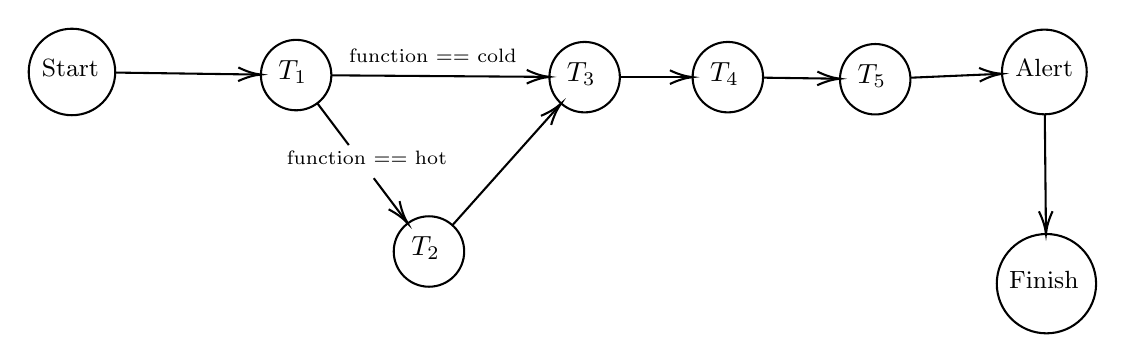
\begin{tikzpicture}[x=0.75pt,y=0.75pt,yscale=-1,xscale=1]
%uncomment if require: \path (0,315); %set diagram left start at 0, and has height of 315


% Text Node
\draw    (211, 93) circle [x radius= 16.97, y radius= 16.97]   ;
\draw (201,84.4) node [anchor=north west][inner sep=0.75pt]    {$T_{1}$};
% Text Node
\draw    (103, 91.5) circle [x radius= 20.84, y radius= 20.84]   ;
\draw (87,84) node [anchor=north west][inner sep=0.75pt]  [font=\small] [align=left] {Start};
% Text Node
\draw    (275, 178) circle [x radius= 16.97, y radius= 16.97]   ;
\draw (265,169.4) node [anchor=north west][inner sep=0.75pt]    {$T_{2}$};
% Text Node
\draw    (350, 94) circle [x radius= 16.97, y radius= 16.97]   ;
\draw (340,85.4) node [anchor=north west][inner sep=0.75pt]    {$T_{3}$};
% Text Node
\draw    (419, 94) circle [x radius= 16.97, y radius= 16.97]   ;
\draw (409,85.4) node [anchor=north west][inner sep=0.75pt]    {$T_{4}$};
% Text Node
\draw    (490, 95) circle [x radius= 16.97, y radius= 16.97]   ;
\draw (480,86.4) node [anchor=north west][inner sep=0.75pt]    {$T_{5}$};
% Text Node
\draw    (571.5, 91.5) circle [x radius= 20.41, y radius= 20.41]   ;
\draw (556,84) node [anchor=north west][inner sep=0.75pt]  [font=\small] [align=left] {Alert};
% Text Node
\draw    (572.5, 193.5) circle [x radius= 23.93, y radius= 23.93]   ;
\draw (553,186) node [anchor=north west][inner sep=0.75pt]  [font=\small] [align=left] {Finish};
% Text Node
\draw (205,128) node [anchor=north west][inner sep=0.75pt]  [font=\scriptsize] [align=left] {function == hot};
% Text Node
\draw (235,79) node [anchor=north west][inner sep=0.75pt]  [font=\scriptsize] [align=left] {function == cold};
% Connection
\draw    (123.84,91.79) -- (192.03,92.74) ;
\draw [shift={(194.03,92.76)}, rotate = 180.8] [color={rgb, 255:red, 0; green, 0; blue, 0 }  ][line width=0.75]    (10.93,-3.29) .. controls (6.95,-1.4) and (3.31,-0.3) .. (0,0) .. controls (3.31,0.3) and (6.95,1.4) .. (10.93,3.29)   ;
% Connection
\draw    (221.21,106.56) -- (236.38,126.71)(248.41,142.69) -- (263.59,162.84) ;
\draw [shift={(264.79,164.44)}, rotate = 233.02] [color={rgb, 255:red, 0; green, 0; blue, 0 }  ][line width=0.75]    (10.93,-3.29) .. controls (6.95,-1.4) and (3.31,-0.3) .. (0,0) .. controls (3.31,0.3) and (6.95,1.4) .. (10.93,3.29)   ;
% Connection
\draw    (286.3,165.34) -- (337.37,108.15) ;
\draw [shift={(338.7,106.66)}, rotate = 131.76] [color={rgb, 255:red, 0; green, 0; blue, 0 }  ][line width=0.75]    (10.93,-3.29) .. controls (6.95,-1.4) and (3.31,-0.3) .. (0,0) .. controls (3.31,0.3) and (6.95,1.4) .. (10.93,3.29)   ;
% Connection
\draw    (366.97,94) -- (400.03,94) ;
\draw [shift={(402.03,94)}, rotate = 180] [color={rgb, 255:red, 0; green, 0; blue, 0 }  ][line width=0.75]    (10.93,-3.29) .. controls (6.95,-1.4) and (3.31,-0.3) .. (0,0) .. controls (3.31,0.3) and (6.95,1.4) .. (10.93,3.29)   ;
% Connection
\draw    (435.97,94.24) -- (471.03,94.73) ;
\draw [shift={(473.03,94.76)}, rotate = 180.81] [color={rgb, 255:red, 0; green, 0; blue, 0 }  ][line width=0.75]    (10.93,-3.29) .. controls (6.95,-1.4) and (3.31,-0.3) .. (0,0) .. controls (3.31,0.3) and (6.95,1.4) .. (10.93,3.29)   ;
% Connection
\draw    (506.96,94.27) -- (549.11,92.46) ;
\draw [shift={(551.11,92.38)}, rotate = 177.54] [color={rgb, 255:red, 0; green, 0; blue, 0 }  ][line width=0.75]    (10.93,-3.29) .. controls (6.95,-1.4) and (3.31,-0.3) .. (0,0) .. controls (3.31,0.3) and (6.95,1.4) .. (10.93,3.29)   ;
% Connection
\draw    (227.97,93.12) -- (331.03,93.86) ;
\draw [shift={(333.03,93.88)}, rotate = 180.41] [color={rgb, 255:red, 0; green, 0; blue, 0 }  ][line width=0.75]    (10.93,-3.29) .. controls (6.95,-1.4) and (3.31,-0.3) .. (0,0) .. controls (3.31,0.3) and (6.95,1.4) .. (10.93,3.29)   ;
% Connection
\draw    (571.7,111.91) -- (572.25,167.57) ;
\draw [shift={(572.27,169.57)}, rotate = 269.44] [color={rgb, 255:red, 0; green, 0; blue, 0 }  ][line width=0.75]    (10.93,-3.29) .. controls (6.95,-1.4) and (3.31,-0.3) .. (0,0) .. controls (3.31,0.3) and (6.95,1.4) .. (10.93,3.29)   ;

\end{tikzpicture}
    \caption{
    حالات اصلی
    }
    \label{fig:diag2}
\end{figure}

از آنجایی که در برخی حالات باید بیش از یک کلاک حضور داشته باشیم یک راه نگه داشتن این حالات و افزودن یک شمارنده برای هر حالت است و راه ساده‌تر که ما اینجا از آن استفاده می‌کنیم زیاد کردن تعداد حالت‌های معادل برای هر حالت است. یعنی مثلا حالتی که قرار است دو کلاک حضور داشته باشد، دو حالت فرعی معادل دارد.
در انتها این حالات فرعی را با مداری به حالت اصلی معادلشان تبدیل می‌کنیم.

حالات فرعی نهایی با شماره‌شان در شمارنده در شکل 
\eqref{fig:diag2}
آمده است.

\begin{figure}[h!]
    \centering
    

\tikzset{every picture/.style={line width=0.75pt}} %set default line width to 0.75pt        

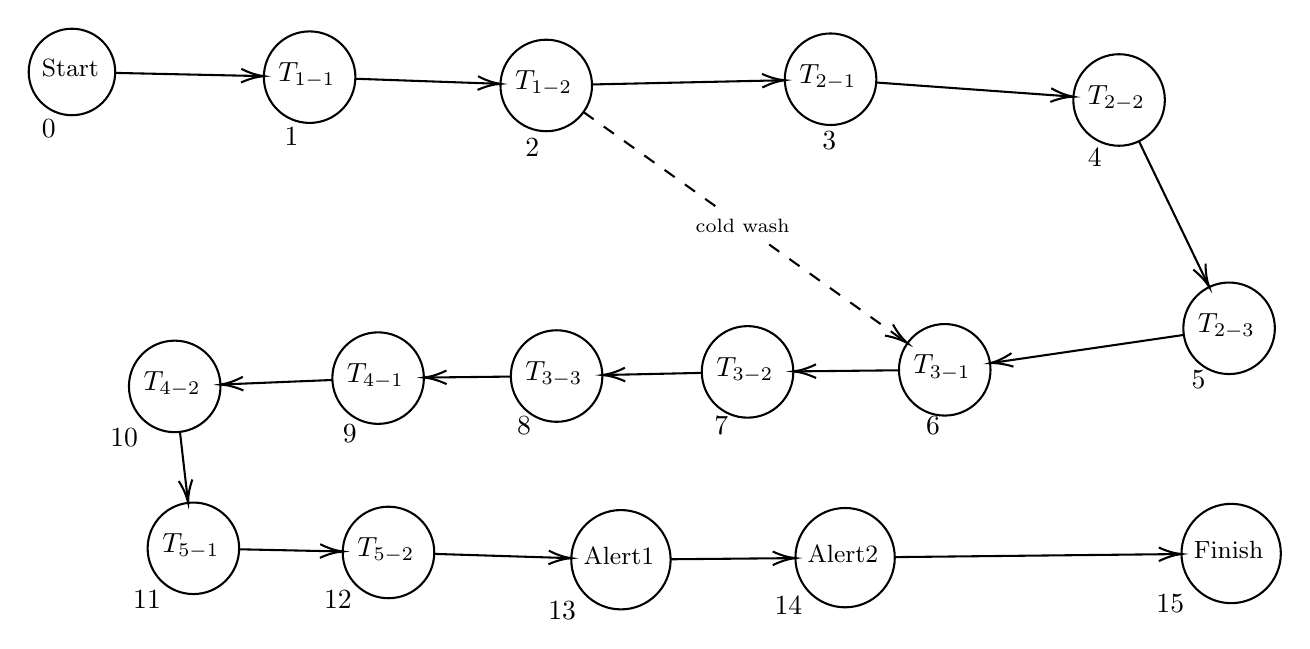
\begin{tikzpicture}[x=0.75pt,y=0.75pt,yscale=-1,xscale=1]
%uncomment if require: \path (0,315); %set diagram left start at 0, and has height of 315


% Text Node
\draw    (157.5, 35) circle [x radius= 22.05, y radius= 22.05]   ;
\draw (141,26.4) node [anchor=north west][inner sep=0.75pt]    {$T_{1-1}$};
% Text Node
\draw    (43, 32.5) circle [x radius= 20.84, y radius= 20.84]   ;
\draw (27,25) node [anchor=north west][inner sep=0.75pt]  [font=\small] [align=left] {Start};
% Text Node
\draw    (271.5, 39) circle [x radius= 22.05, y radius= 22.05]   ;
\draw (255,30.4) node [anchor=north west][inner sep=0.75pt]    {$T_{1-2}$};
% Text Node
\draw    (408.5, 36) circle [x radius= 22.05, y radius= 22.05]   ;
\draw (392,27.4) node [anchor=north west][inner sep=0.75pt]    {$T_{2-1}$};
% Text Node
\draw    (547.5, 46) circle [x radius= 22.05, y radius= 22.05]   ;
\draw (531,37.4) node [anchor=north west][inner sep=0.75pt]    {$T_{2-2}$};
% Text Node
\draw    (600.5, 156) circle [x radius= 22.05, y radius= 22.05]   ;
\draw (584,147.4) node [anchor=north west][inner sep=0.75pt]    {$T_{2-3}$};
% Text Node
\draw    (463.5, 176) circle [x radius= 22.05, y radius= 22.05]   ;
\draw (447,167.4) node [anchor=north west][inner sep=0.75pt]    {$T_{3-1}$};
% Text Node
\draw (342,102) node [anchor=north west][inner sep=0.75pt]  [font=\scriptsize] [align=left] {cold wash};
% Text Node
\draw    (368.5, 177) circle [x radius= 22.05, y radius= 22.05]   ;
\draw (352,168.4) node [anchor=north west][inner sep=0.75pt]    {$T_{3-2}$};
% Text Node
\draw    (276.5, 179) circle [x radius= 22.05, y radius= 22.05]   ;
\draw (260,170.4) node [anchor=north west][inner sep=0.75pt]    {$T_{3-3}$};
% Text Node
\draw    (190.5, 180) circle [x radius= 22.05, y radius= 22.05]   ;
\draw (174,171.4) node [anchor=north west][inner sep=0.75pt]    {$T_{4-1}$};
% Text Node
\draw    (92.5, 184) circle [x radius= 22.05, y radius= 22.05]   ;
\draw (76,175.4) node [anchor=north west][inner sep=0.75pt]    {$T_{4-2}$};
% Text Node
\draw    (195.5, 264) circle [x radius= 22.05, y radius= 22.05]   ;
\draw (179,255.4) node [anchor=north west][inner sep=0.75pt]    {$T_{5-2}$};
% Text Node
\draw    (101.5, 262) circle [x radius= 22.05, y radius= 22.05]   ;
\draw (85,253.4) node [anchor=north west][inner sep=0.75pt]    {$T_{5-1}$};
% Text Node
\draw    (307.5, 267.5) circle [x radius= 23.93, y radius= 23.93]   ;
\draw (288,260) node [anchor=north west][inner sep=0.75pt]  [font=\small] [align=left] {Alert1};
% Text Node
\draw    (415.5, 266.5) circle [x radius= 23.93, y radius= 23.93]   ;
\draw (396,259) node [anchor=north west][inner sep=0.75pt]  [font=\small] [align=left] {Alert2};
% Text Node
\draw    (601.5, 264.5) circle [x radius= 23.93, y radius= 23.93]   ;
\draw (582,257) node [anchor=north west][inner sep=0.75pt]  [font=\small] [align=left] {Finish};
% Text Node
\draw (27,54) node [anchor=north west][inner sep=0.75pt]   [align=left] {0};
% Text Node
\draw (144,58) node [anchor=north west][inner sep=0.75pt]   [align=left] {1};
% Text Node
\draw (260,63) node [anchor=north west][inner sep=0.75pt]   [align=left] {2};
% Text Node
\draw (403,60) node [anchor=north west][inner sep=0.75pt]   [align=left] {3};
% Text Node
\draw (531,68) node [anchor=north west][inner sep=0.75pt]   [align=left] {4};
% Text Node
\draw (581,175) node [anchor=north west][inner sep=0.75pt]   [align=left] {5};
% Text Node
\draw (453,197) node [anchor=north west][inner sep=0.75pt]   [align=left] {6};
% Text Node
\draw (351,197) node [anchor=north west][inner sep=0.75pt]   [align=left] {7};
% Text Node
\draw (256,197) node [anchor=north west][inner sep=0.75pt]   [align=left] {8};
% Text Node
\draw (172,201) node [anchor=north west][inner sep=0.75pt]   [align=left] {9};
% Text Node
\draw (60,203) node [anchor=north west][inner sep=0.75pt]   [align=left] {10};
% Text Node
\draw (71,281) node [anchor=north west][inner sep=0.75pt]   [align=left] {11};
% Text Node
\draw (163,281) node [anchor=north west][inner sep=0.75pt]   [align=left] {12};
% Text Node
\draw (271,286) node [anchor=north west][inner sep=0.75pt]   [align=left] {13};
% Text Node
\draw (380,284) node [anchor=north west][inner sep=0.75pt]   [align=left] {14};
% Text Node
\draw (564,283) node [anchor=north west][inner sep=0.75pt]   [align=left] {15};
% Connection
\draw    (63.83,32.95) -- (133.45,34.47) ;
\draw [shift={(135.45,34.52)}, rotate = 181.25] [color={rgb, 255:red, 0; green, 0; blue, 0 }  ][line width=0.75]    (10.93,-3.29) .. controls (6.95,-1.4) and (3.31,-0.3) .. (0,0) .. controls (3.31,0.3) and (6.95,1.4) .. (10.93,3.29)   ;
% Connection
\draw    (179.54,35.77) -- (247.46,38.16) ;
\draw [shift={(249.46,38.23)}, rotate = 182.01] [color={rgb, 255:red, 0; green, 0; blue, 0 }  ][line width=0.75]    (10.93,-3.29) .. controls (6.95,-1.4) and (3.31,-0.3) .. (0,0) .. controls (3.31,0.3) and (6.95,1.4) .. (10.93,3.29)   ;
% Connection
\draw    (293.55,38.52) -- (384.45,36.53) ;
\draw [shift={(386.45,36.48)}, rotate = 178.75] [color={rgb, 255:red, 0; green, 0; blue, 0 }  ][line width=0.75]    (10.93,-3.29) .. controls (6.95,-1.4) and (3.31,-0.3) .. (0,0) .. controls (3.31,0.3) and (6.95,1.4) .. (10.93,3.29)   ;
% Connection
\draw    (430.5,37.58) -- (523.51,44.27) ;
\draw [shift={(525.5,44.42)}, rotate = 184.11] [color={rgb, 255:red, 0; green, 0; blue, 0 }  ][line width=0.75]    (10.93,-3.29) .. controls (6.95,-1.4) and (3.31,-0.3) .. (0,0) .. controls (3.31,0.3) and (6.95,1.4) .. (10.93,3.29)   ;
% Connection
\draw    (557.07,65.87) -- (590.06,134.33) ;
\draw [shift={(590.93,136.13)}, rotate = 244.27] [color={rgb, 255:red, 0; green, 0; blue, 0 }  ][line width=0.75]    (10.93,-3.29) .. controls (6.95,-1.4) and (3.31,-0.3) .. (0,0) .. controls (3.31,0.3) and (6.95,1.4) .. (10.93,3.29)   ;
% Connection
\draw    (578.68,159.19) -- (487.3,172.53) ;
\draw [shift={(485.32,172.81)}, rotate = 351.69] [color={rgb, 255:red, 0; green, 0; blue, 0 }  ][line width=0.75]    (10.93,-3.29) .. controls (6.95,-1.4) and (3.31,-0.3) .. (0,0) .. controls (3.31,0.3) and (6.95,1.4) .. (10.93,3.29)   ;
% Connection
\draw  [dash pattern={on 4.5pt off 4.5pt}]  (289.45,51.81) -- (354.48,98.21)(378.9,115.63) -- (443.92,162.03) ;
\draw [shift={(445.55,163.19)}, rotate = 215.51] [color={rgb, 255:red, 0; green, 0; blue, 0 }  ][line width=0.75]    (10.93,-3.29) .. controls (6.95,-1.4) and (3.31,-0.3) .. (0,0) .. controls (3.31,0.3) and (6.95,1.4) .. (10.93,3.29)   ;
% Connection
\draw    (441.45,176.23) -- (392.55,176.75) ;
\draw [shift={(390.55,176.77)}, rotate = 359.4] [color={rgb, 255:red, 0; green, 0; blue, 0 }  ][line width=0.75]    (10.93,-3.29) .. controls (6.95,-1.4) and (3.31,-0.3) .. (0,0) .. controls (3.31,0.3) and (6.95,1.4) .. (10.93,3.29)   ;
% Connection
\draw    (346.45,177.48) -- (300.55,178.48) ;
\draw [shift={(298.55,178.52)}, rotate = 358.75] [color={rgb, 255:red, 0; green, 0; blue, 0 }  ][line width=0.75]    (10.93,-3.29) .. controls (6.95,-1.4) and (3.31,-0.3) .. (0,0) .. controls (3.31,0.3) and (6.95,1.4) .. (10.93,3.29)   ;
% Connection
\draw    (254.45,179.26) -- (214.55,179.72) ;
\draw [shift={(212.55,179.74)}, rotate = 359.33] [color={rgb, 255:red, 0; green, 0; blue, 0 }  ][line width=0.75]    (10.93,-3.29) .. controls (6.95,-1.4) and (3.31,-0.3) .. (0,0) .. controls (3.31,0.3) and (6.95,1.4) .. (10.93,3.29)   ;
% Connection
\draw    (168.47,180.9) -- (116.53,183.02) ;
\draw [shift={(114.53,183.1)}, rotate = 357.66] [color={rgb, 255:red, 0; green, 0; blue, 0 }  ][line width=0.75]    (10.93,-3.29) .. controls (6.95,-1.4) and (3.31,-0.3) .. (0,0) .. controls (3.31,0.3) and (6.95,1.4) .. (10.93,3.29)   ;
% Connection
\draw    (95.03,205.91) -- (98.74,238.11) ;
\draw [shift={(98.97,240.09)}, rotate = 263.42] [color={rgb, 255:red, 0; green, 0; blue, 0 }  ][line width=0.75]    (10.93,-3.29) .. controls (6.95,-1.4) and (3.31,-0.3) .. (0,0) .. controls (3.31,0.3) and (6.95,1.4) .. (10.93,3.29)   ;
% Connection
\draw    (123.55,262.47) -- (171.45,263.49) ;
\draw [shift={(173.45,263.53)}, rotate = 181.22] [color={rgb, 255:red, 0; green, 0; blue, 0 }  ][line width=0.75]    (10.93,-3.29) .. controls (6.95,-1.4) and (3.31,-0.3) .. (0,0) .. controls (3.31,0.3) and (6.95,1.4) .. (10.93,3.29)   ;
% Connection
\draw    (217.54,264.69) -- (281.59,266.69) ;
\draw [shift={(283.58,266.75)}, rotate = 181.79] [color={rgb, 255:red, 0; green, 0; blue, 0 }  ][line width=0.75]    (10.93,-3.29) .. controls (6.95,-1.4) and (3.31,-0.3) .. (0,0) .. controls (3.31,0.3) and (6.95,1.4) .. (10.93,3.29)   ;
% Connection
\draw    (331.43,267.28) -- (389.57,266.74) ;
\draw [shift={(391.57,266.72)}, rotate = 179.47] [color={rgb, 255:red, 0; green, 0; blue, 0 }  ][line width=0.75]    (10.93,-3.29) .. controls (6.95,-1.4) and (3.31,-0.3) .. (0,0) .. controls (3.31,0.3) and (6.95,1.4) .. (10.93,3.29)   ;
% Connection
\draw    (439.43,266.24) -- (575.57,264.78) ;
\draw [shift={(577.57,264.76)}, rotate = 179.38] [color={rgb, 255:red, 0; green, 0; blue, 0 }  ][line width=0.75]    (10.93,-3.29) .. controls (6.95,-1.4) and (3.31,-0.3) .. (0,0) .. controls (3.31,0.3) and (6.95,1.4) .. (10.93,3.29)   ;

\end{tikzpicture}
    \caption{
    حالات فرعی
    }
    \label{fig:diag2}
\end{figure}

\section{
پیاده‌سازی سرد و گرم
}
از آنجایی که تنها تخطی ما از شمارش متوالی در حالت شست‌وشوی سرد است از فلیپ‌فلاپ استفاده نکردیم و از یک شمارنده‌ی ساده استفاده کردیم.

برای پیاده‌سازی این تخطی از قابلیت بارگذاری موازی شمارنده استفاده می‌کنیم.
یعنی هنگامی که کارکرد ماشین لباسشویی روی حالت سرد تنظیم شده مدار وقتی به اولین حالت گرم کردن آب می‌رسد درجا به حالت اصلی بعدی می‌پرد (حالت بعدی بارگذاری موازی می‌شود)

از آنجایی که بارگذاری موازی در این شمارنده آنی است و نه با کلاک، باید اولین حالت گرم کردن را در نظر بگیریم نه آخرین حالت قبل از آن را که در شکل
\eqref{fig:load}
مدار آن آورده شده.
ورودی گیت
NAND
یکی حالت تنظیم شده و دیگری حالت دیکد شده‌ی گرم کردن است.

\begin{figure}[h!]
    \centering
    \includegraphics[width=0.5\textwidth]{part1/2.png}
    \caption{
    بارگذاری موازی در شمارنده
    }
    \label{fig:load}
\end{figure}

\section{
پیدا کردن حالات اصلی
}

پس از این که حالات شمارنده را دیکد کردیم به سادگی با OR
کردن حالاتت متناظر با هر حالت اصلی می‌توان متغییر مربوط به آن حالت را یافت که در شکل
\eqref{fig:or}
نحوه‌ی این کار آمده است.
البته می‌توان دیکدر را حذف کرد و با تعدادی گیت اند و نات حالات را مستقیما پیدا کرد که این کار مدار را ساده‌تر می‌کند اما تغییر و خوانایی آن را به شدت می‌کاهد و هر گونه تغییر را در آینده دشوار می‌سازد که در اینجا از این کار پرهیز شده.

\begin{figure}[h!]
    \centering
    \includegraphics[width=0.5\textwidth]{part1/3.png}
    \caption{
    پیدا کردن حالات اصلی از روی حالات دیکد شده‌ی شمارنده
    }
    \label{fig:or}
\end{figure}

\section{
 کلاک با قبلیت دیباگ
}
در شکل
\eqref{fig:clock}
مشاهده می‌کنید که کلاکی با قابلیت دستی (دیباگ) و اتوماتیک
ساخته شده است.

\begin{figure}[h!]
    \centering
    \includegraphics[width=0.5\textwidth]{part1/4.png}
    \caption{
    ساخت کلاک با قابلیت دیباگ (سوییچ بین حالت دستی و اتوماتیک)
    }
    \label{fig:clock}
\end{figure}

\section{
دکمه‌ی استارت هوشمند
}
دکمه استارت نباید باعث شود ماشین لباسشویی پس از ریست شدن دوباره شروع به کار کند.
پس این کلید از نوع
latched
نیست و از نوع
momentary 
است.
اما از طرفی نمی‌توان از مصرف‌کننده خواست که دکمه را به مدت یک کلاک نگه دارد.
بنابراین باید از یک 
latch 
کنترل‌شده
استفاده کرد که وقتی کار به پایان می‌رسد ریست شود.
در شکل \eqref{fig:start}
نحوه‌ی پیاده‌سازی آن نشان داده شده.

در صورتی که مدار در حالت
READY
یا
FINISH
باشد با زدن دکمه‌ی استارت ماشین شروع به شستن می‌کند و با زدن ریست مدار در هر حالتی باشد به حالت
READY
بر می‌گردد که یوزرفرندلی‌ترین ترکیب ممکن برای این دو دکمه است.

\begin{figure}[h!]
    \centering
    \includegraphics[width=0.5\textwidth]{part1/5.png}
    \caption{
    استارت هوشمند
    }
    \label{fig:start}
\end{figure}

\section{
بوق اتمام کار
}
وقتی کار ماشین‌لباسشویی به پایان رسید به مدت دو کلاک مدار بازر چشمک‌زن و چراغ پایان‌کار چشمک می‌زنند.
برای این بوق به کلاک سریع‌تری با مرتبه فرکانسی حدود ۱ هرتز نیاز داریم.

مدت زمان این هشدار دو کلاک در نظر گرفته شده چرا که از ۱۶ حالت شمارنده دو تا باقی‌مانده بود و یک حالت مفت خالی داشتیم.
(البته می‌توان به سادگی خروجی پایان کار و ریست
latch
را از یک حالت بالاتر گرفت و یک حالت شمارنده را هدر داد)
این حالت را می‌توان با تغییری جزئی بعدا برای کارهای جانبی دیگر استفاده کرد.
(مثلا یک حالت تعمیر یا چنین چیزی)

پس از پایان این حالات هشدار پایان کار بوق قطع شده ولی چراغ پایان کار ثابت می‌ماند.

\begin{figure}[h!]
    \centering
    \includegraphics[width=0.5\textwidth]{part1/7.png}
    \caption{
    buzzer
    یا
    بوق پایان کار
    }
    \label{fig:buzzer}
\end{figure}

\section{
گرمکن
}
خروجی
$T_2$
را می‌توان به یک رله وصل کرد تا آن نیز یک گرمکن را به برق شهری وصل کند.

\begin{figure}[h!]
    \centering
    \includegraphics[width=0.5\textwidth]{part1/6.png}
    \caption{
    heater یا گرمکن
    }
    \label{fig:heater}
\end{figure}


\section{
موتور دو سرعته
}

با توجه به شکل
\eqref{fig:motor}
یک موتور دارای دور تند و کند قرار داده شده که دور کند آن به خروجی شست‌و‌شو و دور تند آن به خروجی خشک‌کن وصل است.

\begin{figure}[h!]
    \centering
    \includegraphics[width=0.5\textwidth]{part1/8.png}
    \caption{
    موتور دور تند و کند
    }
    \label{fig:motor}
\end{figure}


\section{مدار نهایی}
\begin{figure}[h!]
    \centering
    \includegraphics[width=\textwidth]{part1/1.png}
    \caption{
    شکل مدار
    }
    \label{fig:final}
\end{figure}